% 图 8.11 自旋梯子：(a) 两腿梯 (b) 三腿梯 (c) 两腿梯单态基态
% (d) 两空穴分处两横档（破坏 2 个单态）(e) 两空穴同横档（只破坏 1 个单态）
\documentclass[tikz,border=5pt]{standalone}
\usetikzlibrary{arrows.meta}
\usepackage{amsmath}
\usepackage{bm}
\usepackage{fontspec}
\setmainfont{Times New Roman}
\begin{document}
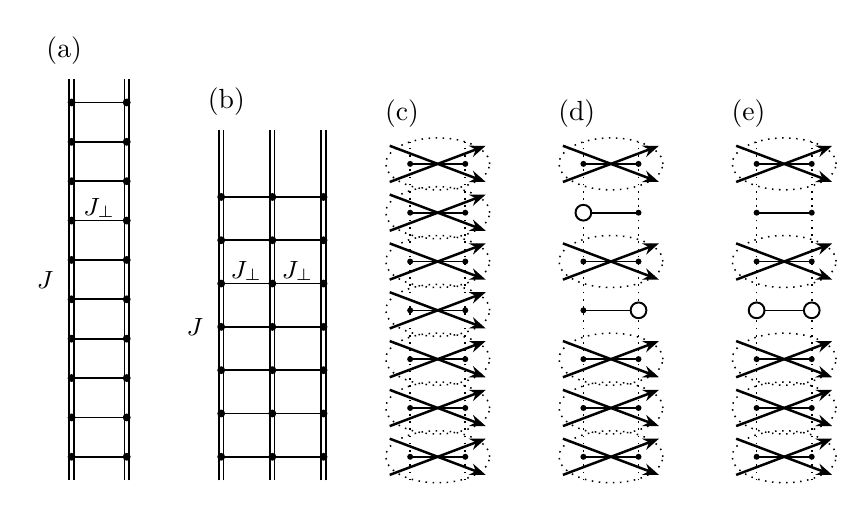
\begin{tikzpicture}[line width=0.8pt,>=Stealth,
  sing/.style={line width=0.9,-{Stealth[length=2.0mm,width=1.5mm]}}]
% ---------- (a) two-leg ladder ----------
\begin{scope}[shift={(0,0)}]
  \foreach \y in {0,0.5,...,4.5}{ \draw[line width=0.6] (0.4,\y) -- (1.1,\y); }
  \draw[line width=0.55] (0.37,-0.3) -- (0.37,4.8);
  \draw[line width=0.55] (0.43,-0.3) -- (0.43,4.8);
  \draw[line width=0.55] (1.07,-0.3) -- (1.07,4.8);
  \draw[line width=0.55] (1.13,-0.3) -- (1.13,4.8);
  \foreach \y in {0,0.5,...,4.5}{
    \fill (0.4,\y) circle (0.05); \fill (1.1,\y) circle (0.05);}
  \node at (0.75,3.16) {\small $J_\perp$};
  \node[left] at (0.30,2.25) {\small $J$};
  \node[anchor=south west] at (-0.05,4.85) {(a)};
\end{scope}
% ---------- (b) three-leg ladder ----------
\begin{scope}[shift={(2.1,0)}]
  \foreach \y in {0,0.55,...,3.85}{
    \draw[line width=0.6] (0.2,\y) -- (0.85,\y);
    \draw[line width=0.6] (0.85,\y) -- (1.5,\y);}
  \foreach \x in {0.17,0.23,0.82,0.88,1.47,1.53}{ \draw[line width=0.55] (\x,-0.3) -- (\x,4.15); }
  \foreach \y in {0,0.55,...,3.85}{
    \fill (0.2,\y) circle (0.05); \fill (0.85,\y) circle (0.05); \fill (1.5,\y) circle (0.05);}
  \node at (0.52,2.36) {\small $J_\perp$};
  \node at (1.17,2.36) {\small $J_\perp$};
  \node[left] at (0.10,1.65) {\small $J$};
  \node[anchor=south west] at (-0.1,4.2) {(b)};
\end{scope}
% ---------- (c) two-leg ladder ground state: rung singlets ----------
\begin{scope}[shift={(4.3,0)}]
  \draw[dotted,line width=0.6] (0.4,-0.3) -- (0.4,4.0);
  \draw[dotted,line width=0.6] (1.1,-0.3) -- (1.1,4.0);
  \foreach \y in {0,0.62,...,3.72}{
    \draw[line width=0.6] (0.4,\y) -- (1.1,\y);
    \fill (0.4,\y) circle (0.038); \fill (1.1,\y) circle (0.038);
    \draw[dotted,line width=0.55] (0.75,\y) ellipse [x radius=0.66, y radius=0.33];
    \draw[sing] (0.14,{\y-0.23}) -- (1.36,{\y+0.23});
    \draw[sing] (0.14,{\y+0.23}) -- (1.36,{\y-0.23});}
  \node[anchor=south west] at (-0.05,4.05) {(c)};
\end{scope}
% ---------- (d) two holes on different rungs: two singlets broken ----------
\begin{scope}[shift={(6.5,0)}]
  \draw[dotted,line width=0.6] (0.4,-0.3) -- (0.4,4.0);
  \draw[dotted,line width=0.6] (1.1,-0.3) -- (1.1,4.0);
  \foreach \y in {0,0.62,...,3.72}{
    \draw[line width=0.6] (0.4,\y) -- (1.1,\y);
    \fill (0.4,\y) circle (0.038); \fill (1.1,\y) circle (0.038);}
  \foreach \y in {0,0.62,1.24,2.48,3.72}{
    \draw[dotted,line width=0.55] (0.75,\y) ellipse [x radius=0.66, y radius=0.33];
    \draw[sing] (0.14,{\y-0.23}) -- (1.36,{\y+0.23});
    \draw[sing] (0.14,{\y+0.23}) -- (1.36,{\y-0.23});}
  % holes: rung 2 (left leg) and rung 4 (right leg), counted from the top
  \draw[fill=white,line width=0.7] (0.4,3.10) circle (0.10);
  \draw[fill=white,line width=0.7] (1.1,1.86) circle (0.10);
  \node[anchor=south west] at (-0.05,4.05) {(d)};
\end{scope}
% ---------- (e) two holes on the same rung: one singlet broken ----------
\begin{scope}[shift={(8.7,0)}]
  \draw[dotted,line width=0.6] (0.4,-0.3) -- (0.4,4.0);
  \draw[dotted,line width=0.6] (1.1,-0.3) -- (1.1,4.0);
  \foreach \y in {0,0.62,...,3.72}{
    \draw[line width=0.6] (0.4,\y) -- (1.1,\y);
    \fill (0.4,\y) circle (0.038); \fill (1.1,\y) circle (0.038);}
  \foreach \y in {0,0.62,1.24,2.48,3.72}{
    \draw[dotted,line width=0.55] (0.75,\y) ellipse [x radius=0.66, y radius=0.33];
    \draw[sing] (0.14,{\y-0.23}) -- (1.36,{\y+0.23});
    \draw[sing] (0.14,{\y+0.23}) -- (1.36,{\y-0.23});}
  % both holes share the middle rung
  \draw[fill=white,line width=0.7] (0.4,1.86) circle (0.10);
  \draw[fill=white,line width=0.7] (1.1,1.86) circle (0.10);
  \node[anchor=south west] at (-0.05,4.05) {(e)};
\end{scope}
\end{tikzpicture}
\end{document}
